\documentclass[11pt]{article}

% Packages to use
\usepackage[margin=1in]{geometry}
\usepackage{microtype}
\usepackage{booktabs}
\usepackage{hyperref}
\usepackage{graphicx}

\title{
	Feed grain price: Data cleaning and analysis \\
	\Large BIOS 7400 final project, Spring 2022
}
\author{Zane Billings}
\date{2022-05-06}

\begin{document}

\maketitle

\section*{Dataset}

Even before the discovery of agriculture, humans have eaten grains. When ancient
humans in the fertile crescent first cultivated cereal crops and abandoned their
hunter-gatherer lifestyles for farming around 9000 BCE \cite{zeder2011}, they
set in motion a chain of events which ultimately culminated in this report.
From their humble origins at the foundation of modern human society, feed grains
travelled across the globe and remain an economic and dietary staple today. In
the modern monoculture crop economy, millions of tons of raw cereal grains
are produced monthly \cite{fao}. In addition to their human comestibility,
over a third of all agricultural crops grown worldwide are used for animal
feed \cite{cassidy2013}.

In particular, the United States produces enough feed grain to feed 800 million
humans, if use were changed, according to one researcher \cite{chron}.
Cereals of particular importance to the economy of the United States are corn
(maize), barley, oats, and sorghum, with corn accounting for around 95\% of all
feed grain production \cite{ataglance}. The United States Department of
Agriculture (USDA) tracks the total acreage planted and harvested of all four
of these grains yearly, and records a great deal of information about their
price. Overall, there is a direct link between feed grain prices and
grain commodity futures, which are strongly affected by USDA forecasts
\cite{arnade2021}. As commodity futures are valuable in themselves, and are
additionally linked to other economic indicators and investments
\cite{irwin2011}, forecasting grain prices as recorded by the USDA can provide
valuable economic information. We utilize USDA data as well as other publicly
available information to build understanding of feed grain prices, and perform
simple analyses which may inform future prices.

In order to analyze trends in USDA feed grains prices, we collected several
data sets and performed a variety of statistical analyses, which we describe
here. All raw data, the \texttt{.sas7bdat} cleaned data file, and all SAS code
used for this project, along with relevant SAS logs and output are provided on
the public GitHub page for this project:
\href{https://github.com/wzbillings/SAS-Grain-Prices}{\texttt{wzbillings/SAS-Grain-Prices}}.

\section*{Data management}

We used SAS version 9.4 (SAS Institute, Cary, NC) for all data management and
statistical analyses. Specifically, we accessed SAS using the SAS on Demand for
Academics SAS Studio platform. All four of the data sets listed in the previous
system were imported into SAS.

\subsubsection*{Feed grains data}

The main data set for our analysis was the
\href{https://www.ers.usda.gov/data-products/feed-grains-database/}{USDA feed
	grains database}. The USDA collects data from across the United States on a
monthly basis, and publicly distributes these data. The majority of the data
are concerned with the four main feed crops discussed earlier. Although the
complete feed grains database contains a lot of useful information, for our
analysis we will limit ourselves to only one section of the data base: the
``U.S. acreage, production, yield, and farm price'' section. These data are
collected on an annual basis and released in the USDA's feed yearbook.
Beginning in the 1866 fiscal (market) year, information on the total harvested
acreage, production in bushels, yield of grain per harvested acre, and weighted
farm average price were collected for corn, barley, and oats. The price of
sorghum was additionally collected beginning in the 1919 fiscal year.

While the other variables are mainly self-explanatory (referring to quantities
reported by individual farmers and aggregated by the USDA), the weighted farm
average price is based on the monthly price recieved by farmers, weighted by
the amount of grain put to market that month. The price does not take any other
financial information into consideration, and is reported in USD per bushel.
Beginning in 1926, the total planted acerage was recorded for corn, oats, and
barley, in order to determine the amount of planted grain which was actually
harvested. Beginning in 1929, the planted and harvested acreage, production and
yield for sorghum were collected as well. Finally, the annual loan rate (USD
per bushel of grain) was collected from 1950 onwards, but is sporadic in the
early years of collection. By 1977, loan rate was being collected regularly for
all four grains.

We hypothesize that one of harvested acres, production, or yield is the main
predictor of commodity price in these data (note that since yield is a function
of harvested acres and production, these three variables form a collinear set
all together, but any two of these variables are not collinear). However, we
believe that other external factors will influence the price of feed grains,
which we will describe later in this section.

To access the the feed grains data set, we downloaded the original Microsoft
Excel workbook from the previously listed USDA webpage. The Excel workbook is
incredibly messy, and thus \texttt{PROC IMPORT} was unsuitable for our
purposes. So, we saved the sheet of interest as a comma-separated value (CSV)
file, which we were able to import into SAS using a \texttt{DATA} step. Due to
the way Microsoft Excel formats exported CSV files, we had to import all values
as character variables and use manual pointer controls to skip empty lines in
the data set. We then used SAS to fill down missing values for which grain was
being recorded (the value was listed once at the beginning of the time series,
so for storing data in SAS it is necessary to fill in missing values for the
entire time series).

The years are reported as fiscal years, in the format 1866/67. We created a new
numeric year variable by taking the first four digits of this variable. Since
the relative spacing of the time series remains the same, it does not matter if
we chose 1866 or 1867 (for example) to recode the year--while the forecasts
might be slightly asynchronous and the final predictions would need to be
recoded to the fiscal years originally listed, recoding the time variable in
this way will not affect our results. We could have recoded the year as 1, 2,
3, etc., with no issues as long as the spacing is unchanged.

We used SAS to parse the numeric variables which were previously interpreted as
character variables during the \texttt{INPUT} statement execution. Since some
of the numbers were exported from Excel with commas as place-value seperators,
we had to use the \texttt{comma\textit{w}.\textit{d}} informat to parse these
values. We also calculated the percent increase in price from the previous
year, and the log (base10) price. Finally, we assigned descriptive labels to
the variable names. Short variable names are easier to use in practice, but the
labels ensure that the code and results remain readable.

\subsection*{Temperature data}

Since global climate change (particularly anthropogenic climate change) is
known to influence weather patterns and agricultural yields, we also wanted to
use a measure of global climate change in our model. However, measures of
global climate change require global weather or climate data, which was largely
unavailable until the 20th century. However, NASA reports the land-ocean
temperature index (measured in deviation from a baseline period) for all years
since 1880 as part of their \href{https://data.giss.nasa.gov/gistemp/}{GISTEMP}
program, so we downloaded these data as well.

The NASA temperature data, downloaded from the GISTEMP project website as a
plain text (space-delimited) file, was by far the most difficult data set to
read into SAS correctly. The data contained multiple header rows and blank rows
within the same file. So, we only used the pointer input mode (single trailing
\texttt{@}) for the \texttt{INPUT} step here, bringing the next line of the
file into the memory buffer and manipulating that manually. First, we scanned
the first detectable word of the input file to determine if it was a numeric
digit or not. All of the actual data lines in the file begin with a year
number, so we discarded any line which did not begin with a digit from the
memory buffer, and then brought the next file line in. Using this strategy
successfully removed both additional header rows and blank rows from the data
set.

Even among the valid data rows, we had to solve another issue: missing values
were noted as either ``\texttt{****}'' or ``\texttt{***}'' in the data, which
generated warning messages when attempting to read the data in as numeric
variables. Fortunately, we could ignore all ``\texttt{***}'' as they were in
columns we did not need (pre-computed averages). We used the SAS function
\texttt{TRANSTRN} to replace all ``\texttt{****}'' with a single period in the
current memory buffer, as a period represents a numeric missing value in SAS.
Finally, we calculated the annual mean from the monthly temperature
observations. We divided the mean by 100 to put the values in units of degrees
Celsius, and rounded to the nearest hundreth of a degree to avoid overstating
the precision of the measurements. Again, we assigned descriptive labels.

\subsection*{Inflation data}

As the value of one USD has steadily decreased since 1866, we believe inflation
is also an important predictor of price. We downloaded inflation data from
\href{https://in2013dollars.com}{in2013dollars}, an online project which uses
data from the United States Bureau of Labor Statistics and historical data to
calculate the value of the U.S. dollar adjusted for inflation, going as far
back as 1665. We set the inflation-adjusted USD value to be relative to 1866,
the first year of feed grain price data collection. The data also contain the
inflation rate for each year.

The inflation data was easy to import into SAS using standard methods. The
only manipulation we made to this data set was to compute the buying power of
one current US dollar in 1866 (buying power, for short) by taking the
multiplicate inverse of the relative worth of one 1866 dollar in the current
year, as the buying power can be easier to interpret relative to the 1866
baseline. We rounded our calculation to the nearest cent and assigned
descriptive labels to all variables.

\subsection*{Presidential party data}

Finally, as a personal curiosity, we were interested in whether American
politics had a strong effect on feed grain prices over time. We downloaded a
data set of presidential party by year from the publication
\href{https://www.theguardian.com/news/datablog/2012/oct/15/us-presidents-listed#data}{The
	Guardian} for convenience.

The Presidential data was easy to import using a \texttt{DATA} step, requiring
no special or complicated manipulations like the previous data sets. However,
there were two issues we had to address with these data. First, the downloaded
data set only went to 2013. So we used publicly available
data to fill in the president names and political parties for the years
2014--2022. Second, we recoded the party of two Presidents in the data set:
Abraham Lincoln and Andrew Johnson ran on the National Union party ticket after
the end of the American Civil War, but Abraham Lincoln is typically regarded as
a republican and Andrew Johnson as a democrat. Recoding Andrew Johnson's
political party allowed us to avoid having a small National Union subgroup with
virtually no statistical power in our analyses. We assigned descriptive labels
as usual.

\subsection*{Cleaned SAS dataset}

In order to create a unified clean SAS dataset, we needed to combine all four
of the datasets of interest. First, we wrote a SAS macro to sort an arbitrary
number of datasets, and used this macro to sort all four of our datasets by
year. Then, we conducted a one-to-many merge of the four datasets by year (note
that this is a one-to-many merge because there are up to four observations for
each year, one for each grain, in the feed grains data). We did not include any
observations in the merged dataset which were for years before 1866 (included
in the presidential data) or after 2022 (not included, but we added this
threshold just in case there were any issues). Both the upper and lower year
limits can be easily adjusted as macro variables at the beginning of the SAS
code if a different range is desired. Finally, we sorted the cleaned dataset by
grain type and then year. The final dataset is saved as
\texttt{grains.sas7bdat} and is available as part of this project.

\section*{Analysis}

For our statistical analyses, we used log of price (base 10,
but we will just say log for simplicity) as the main outcome, as price had a
wide range. The numerical  covariates of interest were planted acerage,
harvested acerage, loan rate,  production, yield, inflation rate, buying power,
value of one 1866 dollar in  current year, and temperature anomaly. The only
categorical covariate of interest was the president's political party. Note
that some covariates were missing at the beginning of the time series. Missing
values were pairwise deleted for each analysis as necessary. Since these models
are predictive, we are not concerned with potential bias induced by pairwise
deletion.

Our first statistical analyses were visual. We used the SAS procedures
\texttt{PROC SGPLOT}, \texttt{PROC SGPANEL}, and
\texttt{PROC SGSCATTER} in order to create plots of log price vs. time, vs. all
covariates (without respect to time). We also plotted the time series of each
covariate of interest, and created a scatterplot matrix of all covariates.
Finally, we also plotted the time series of log price with points colored by
President's political party. The plot of the time series of log price is shown
in Figure \ref{fig:timeseries}. The plot matrices are not shown.

\begin{figure}[!ht]
	\centering
	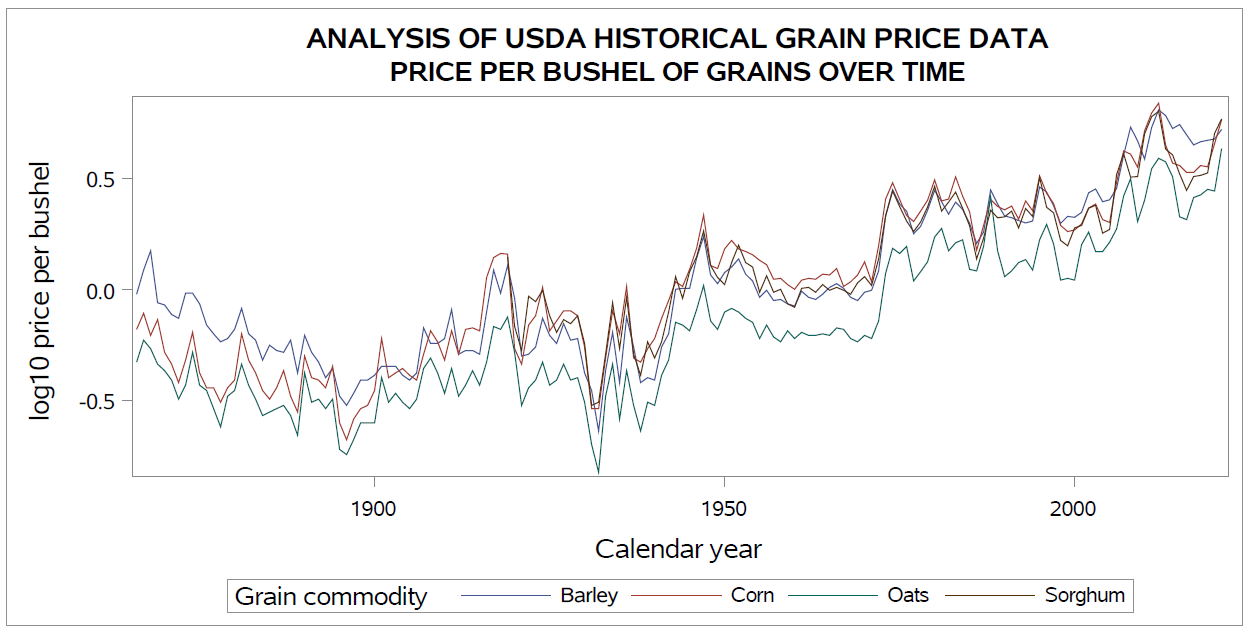
\includegraphics[height=3in]{../figs/timeseries.png}
	\caption{The time series of log10 feed grain prices per year since 1866.
	The series have similar patterns, but varying magnitudes.}
	\label{fig:timeseries}
\end{figure}

For formal statistical analyses, we used \texttt{PROC UNIVARIATE} to obtain
descriptive statistics of log price for each grain, we used \texttt{PROC CORR}
to obtain Pearson and Spearman correlation matrices for log price and all
numeric covariates, and we used \texttt{PROC MEANS} to obtain means, standard
errors, and medians, for log price for each value of president's party (in the
class statement), stratified by grain (in the by statement). Univariate
statistics for log price are shown in Table \ref{tab:univar}.

\begin{table}
	\centering
	\begin{tabular}{rllllll}
		\toprule
		Grain & Mean & St. Dev. & Median & IQR & Min & Max \\
		\midrule
		Barley & 0.029 & 0.342 & -0.029 & 0.567 & -0.638 & 0.808 \\
		Corn & 0.018 & 0.362 & 0.033 & 0.639 & -0.678 & 0.838 \\
		Oats & -0.179 & 0.338 & -0.222 & 0.544 & -0.824 & 0.633 \\
		Sorghum & 0.167 & 0.290 & 0.146 & 0.388 & -0.523 & 0.801 \\
		\bottomrule
	\end{tabular}
	\caption{Univariate statistics for log10 grain price.}
	\label{tab:univar}
\end{table}

Based on the univariate analyses and time series plots, we determined that all
analyses should be stratified by grain--in essence, a separate model should be
fitted for each grain type. From the correlation matrices (not shown) we
determined that several covariates were highly correlated and we decided to
analyze the following set of covariates: acres of grain harvested, production
of grain, inflation rate, buying power, presidential party, temperature
anomaly, and year.

After calculating descriptive statistics, we also created simple linear
regression models (using \texttt{PROC GLM} which can handle multiple
categorical variables) of log price predicted by all covariates individually.
In addition to the selected covariate for each model, grain and an interaction
term between grain and the covariate were included. (Note that this produces
the same effect as stratifying the regression model by grain.) The $R^2$ value
for each model is shown in Table \ref{tab:SLR}. All models had global $F$-tests
significant at a 0.001 alpha level.

\begin{table}[h!]
	\centering
	\begin{tabular}{rl}
		\toprule
		Covariate & $R^2$  \\
		\midrule
		Grain only & 11.02\%  \\
		Acerage planted & 52.40\%  \\
		Production & 43.44\%  \\
		Inflation rate & 27.24\% \\
		Temperature anomaly & 63.88\% \\
		Buying power & 79.99\% \\
		Calendar year & 77.13\% \\
		President's party & 12.29\% \\
		\bottomrule
	\end{tabular}
	\caption{From the $R^2$ values for simple linear regression, the most
	important features appear to be calendar year, buying power, and
	temperature anomaly.}
	\label{tab:SLR}
\end{table}

Then, we built full linear regression models using the maximum available
(non-missing) data, which predicted log price by the selected covariates. All
covariates were
allowed to interact with grain, and a main effect of grain was included
(equivalent to stratification by grain). We built a second model including the
temperature anomaly (and interaction with grain)--this model had less data
points for estimation, as temperature anomaly was not collected until 1880. We
compared the two models with AIC, and the model with lower AIC was used in a
repeated measures model.

As the 1866 model (without temperature anomaly) was better, we used this model
statement to fit a generalized least squares model using \texttt{PROC MIXED}
which allowed for exchangeable (compound symmetric) correlations between time
points. We removed president's political party from this ``final'' regression
model as there was no evidence suggesting an effect for this variable. The
groupwise Wald-type chi-squared tests were all significant at a 0.01
significant level, with the exception of grain production. We additionally
obtained the parameter estimates and confidence intervals, but they are not
shown. All linear model AICs are shown in Table \ref{tab:AIC}. The AIC for the
generalized least squares model is lower than the OLS model, indicating that
allowing for correlation does not provide any additional information when
taking the additional estimated parameters into account.

\begin{table}
	\centering
		\begin{tabular}{rl}
		\toprule
		Model & AIC \\
		\midrule
		1866 linear model & -642 \\
		1880 linear model & -609 \\
		GLS linear model  & -637 \\
		\bottomrule
	\end{tabular}
	\caption{The AICs for the linear models. The original 1866 linear model
	without controlling for correlation provided the best fit.}
	\label{tab:AIC}
\end{table}

Finally, we built a simple ARIMA forecasting model and compared the AIC of this
model to our regression models. We used the SCAN method (not shown) to identify
candidate ARIMA models, which are listed as columns in Table \ref{tab:ARIMA}.
AIC was used for model selection and the AICs are shown in \ref{tab:ARIMA}.
Based on AIC, we observed that the ARIMA(1, 1, 1) model provided little
advantage over the ARIMA(0, 1, 0) (random walk) model, so we did not proceed to
the forecasting stage.

\begin{table}[h!]
	\centering
	\begin{tabular}{rllllllll}
		\toprule
		      & \multicolumn{8}{c}{ARIMA model} \\
		        \cmidrule{2-9}
		Grain & 1,0,0 & 2,0,0 & 0,1,0 & 1,0,1 & 1,1,0 & 1,1,1 & 0,0,0 & 0,1,0 \\
		\midrule
		Barley  & -291 & -289 & -56 & -289 & -288 & -292 & 109 & -289 \\
		Corn    & -248 & -246 & -25 & -246 & -245 & -254 & 126 & -247 \\
		Oats    & -263 & -261 & -56 & -261 & -260 & -270 & 106 & -262 \\
		Sorghum & -159 & -157 & -55 & -157 & -155 & -159 &  38 & -157 \\
		\bottomrule
	\end{tabular}
	\caption{AIC values for various fitted ARIMA models. The ARIMA(1, 1, 1)
	model appears to fit best for all grains. Note 	that the ARIMA(0, 1, 0)
	model, which is equivalent to a random walk, fits essentially as well as
	this model. Comparing the ARIMA models with the nondifferenced ARMA models
	using AIC is not strictly appropriate, but we do so here for simplicity
	with the constraints of the SAS procedure.}
	\label{tab:ARIMA}
\end{table}

\section*{Conclusions}

Overall, we were not successful in generating accurate forecasts for the
time-series data using ARIMA. The ARIMA models are inconclusive about whether
an autoregressive trend is present in the time series, as a random walk model
fits the data very well. However, the generalized least squares regression
analysis also suggests that several covariates may be useful in predicting
grain prices, so a potential autoregressive component to the trend is not the
only important source of information. The random walk model appeared to fit
better than the best regression model, but the AICs are not truly comparable
and a universal measure of goodness-of-fit such as $R^2$ or RMSE would be more
appropriate. Building better regression models, or
more sophisticated forecasting models, using these same data may be of interest
in the future. We also recommend analysis of cross-correlation functions
between covariates and log price in a future analysis to inform modeling.

\newpage
\bibliographystyle{unsrt}
\bibliography{refs}

\end{document}